\documentclass[usenames,dvipsnames,aspectratio=169,10pt]{beamer}
%\usetheme{default}
\usetheme[progressbar=frametitle]{metropolis}

\def \EXAMPLEVERSION {1} % 1 for examples, 2 to hide examples (they are in textbook), 3 to hide examples but leave blank slide

\def \SCHOOLVERSION {1} % 1 for neutral, 2 for ISEP

%\documentclass[12pt]{book}
\usepackage{amsfonts}
\usepackage{amsmath}
\usepackage{amssymb}
\usepackage{graphicx}
\usepackage[authoryear]{natbib}
%\usepackage[margin=2.5cm]{geometry}
%\usepackage{hyperref}
\usepackage[font=footnotesize]{caption}
\usepackage{float}
\usepackage{caption}
\usepackage{subcaption}
\usepackage{setspace}
\usepackage{cleveref}
\usepackage{lscape}
\usepackage{multirow}
\usepackage{nicematrix}

% for tikz
\usepackage{tikz}
\usetikzlibrary{angles, arrows.meta, calc, quotes}
\usetikzlibrary{decorations.pathreplacing,calligraphy}
\usetikzlibrary{patterns}
\usetikzlibrary{bending,matrix,positioning}
\usetikzlibrary{arrows, fit, shapes, backgrounds}

\usepackage{tikz-3dplot}
\usepackage{xcolor}


% for red line canceling diagonally
\usepackage{cancel}
\renewcommand{\CancelColor}{\color{red}}

\captionsetup{font=small,labelfont=bf,singlelinecheck=off,margin=2cm,justification=justified}
\numberwithin{equation}{section}

\newcommand{\defbox}[3]
	{
		\vspace{0.5cm} 
		\noindent \fbox{\begin{minipage}{\linewidth}
		\textbf{{#1}DEFINITION{#2}} #3
		\end{minipage}}
		\vspace{0.5cm}
	}
	
	
\newcommand{\defnobox}[3]
	{
		\vspace{0.5cm} 
		\noindent \begin{minipage}{\linewidth}
		\textbf{{#1}DEFINITION{#2}} #3
		\end{minipage}
		\vspace{0.5cm}
	}
	
%%%% To get a nice colourful box around an equation
\newcommand*{\colourboxed}{}
\def\colourboxed#1#{%
  \colourboxedAux{#1}%
}
\newcommand*{\colourboxedAux}[3]{%
  % #1: optional argument for color model
  % #2: color specification
  % #3: formula
  \begingroup
    \colorlet{cb@saved}{.}%
    \color#1{#2}%
    \boxed{%
      \color{cb@saved}%
      #3%
    }%
  \endgroup
}


%%%%%% COLOURS %%%%%%%%%%
\definecolor{airforceblue}{rgb}{0.36, 0.54, 0.66}
\definecolor{battleshipgrey}{rgb}{0.52, 0.52, 0.51}
\definecolor{brightmaroon}{rgb}{0.76, 0.13, 0.28}
\definecolor{nicegreen}{RGB}{133, 204, 111}

% isep colours
\definecolor{isepblue1}{RGB}{0, 97, 161}      % teinte à 100%
\definecolor{isepblue2}{RGB}{77, 144, 189}    % teinte à 70%
\definecolor{isepblue3}{RGB}{179, 208, 227}   % teinte à 30%
\definecolor{iseporange1}{RGB}{244, 161, 0}   % teinte à 100%
\definecolor{iseporange2}{RGB}{234, 189, 100} % teinte à 70%
\definecolor{iseporange3}{RGB}{252, 227, 179} % teinte à 30%
%%%%%%%%%%%%%%%%

% beamer stuff
\setbeamertemplate{navigation symbols}{}
\setbeamersize{text margin left=1.0cm,text margin right=1.0cm}
\setbeamercolor{background canvas}{bg=white}

\ifnum \SCHOOLVERSION = 2
	%%%% ISEP COLOURS %%%%
	\setbeamercolor{frametitle}{bg=isepblue1, fg=white}
	\setbeamercolor{progress bar}{fg=iseporange1}
	\setbeamercolor{itemize item}{fg=iseporange1,bg=iseporange1}
	%%%%%%%%%%%%%%%%%%%%%%
\fi

\setbeamerfont{frametitle}{family=\fontfamily{qag}\selectfont} % choose font for frame titles
\setbeamerfont{title}{family=\fontfamily{qag}\selectfont} % choose font for title
\setbeamerfont{subtitle}{family=\fontfamily{qag}\selectfont} % choose font for subtitle
\setbeamerfont{section title}{family=\fontfamily{qag}\selectfont} % choose font for titles
%\fontfamily{qag}\selectfont %choose font for main text % put after begin{document}

% to make the progress bar a little thicker
\makeatletter
\setlength{\metropolis@titleseparator@linewidth}{1.5pt}
\setlength{\metropolis@progressonsectionpage@linewidth}{1.5pt}
\setlength{\metropolis@progressinheadfoot@linewidth}{1.5pt}
\makeatother

\begin{document}

\title{Linear Algebra}
\subtitle{System of Linear Equations}
\author{Andrew Lehmann}
\ifnum \SCHOOLVERSION = 2
	\institute{\'{E}cole d'ing\'{e}nieurs du num\'{e}rique}
\fi
\date{\textit{Last updated: \today}}

% logo of university
\ifnum \SCHOOLVERSION = 2
	\titlegraphic{\includegraphics[width=3cm]{/home/andrew/Dropbox/ISEP/admin/logo-isep-2023.png} }
\fi

\begin{frame}
\titlepage
\end{frame}


%%%%%%%%%%%%%%%%%%%%%%%%%%%%%%%%%%%%%%%%%%%%%%%%%%%%%%%%%%%%%%%%%%%%%%%%
\begin{frame}
\frametitle{Example - Electronic circuits}

\begin{figure}[H]
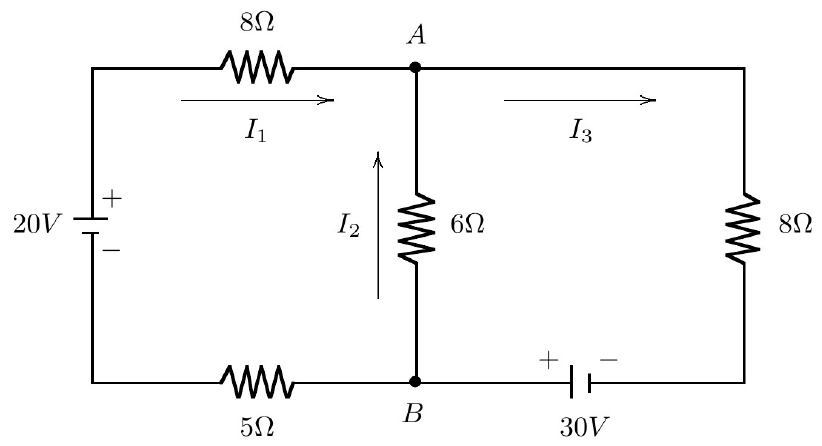
\includegraphics[width=0.6\textwidth]{example_circuit.png}
\end{figure}

Kirchhoff's laws give a system of equations: 
\begin{align*}
\begin{matrix}
I_1 + I_2 - I_3 = 0 \\
13I_1 - I_2 = 20 \\
6I_2 + 8I_3 = 30
\end{matrix}
\qquad
\begin{matrix}
\text{``techniques''} \\
\implies
\end{matrix}
\qquad
\begin{matrix}
I_1 =2\text{ A} \\
I_2 =1\text{ A} \\
I_3 =3\text{ A}
\end{matrix}
\end{align*}

\end{frame}
%%%%%%%%%%%%%%%%%%%%%%%%%%%%%%%%%%%%%%%%%%%%%%%%%%%%%%%%%%%%%%%%%%%%%%%%



%%%%%%%%%%%%%%%%%%%%%%%%%%%%%%%%%%%%%%%%%%%%%%%%%%%%%%%%%%%%%%%%%%%%%%%%
\begin{frame}
\frametitle{Example - Intersection of lines}

Lines form a simple system of equations if we want to find their intersection. For example:

\begin{figure}[H]
\begin{tikzpicture}[line cap=round, line join=round, >=Triangle,scale=1]
	% coordinate system
	\coordinate (O) at (0,0); 
	\draw[->] (-1.5, 0) -- (3,0) node[right] {$x$};
	\draw[->] (0, -0.5) -- (0,3) node[above] {$y$};
	
	% straight lines y= x/2 + 1 and y= -x/3 + 2
	\draw[-,very thick,brightmaroon] (-1,0.5)--(2.5,2.25) node[right,black] {$y= \dfrac{1}{2}x + 1$};
	\draw[-,very thick,nicegreen] (-1,2.33)--(2.5,1.17) node[below right,black] {$y= -\dfrac{1}{3}x + 2$};
	
	\draw[->,black] (1.3,2.5)--(1.21,1.68) node[pos=0,above,black,scale=0.8] {$(x,y)=\left(\dfrac{6}{5},\dfrac{8}{5}\right)$};

	\end{tikzpicture}
\end{figure}

These two equations are simultaneously true at just 1 point, where the two lines overlap: $x=6/5$, $y=8/5$.

\end{frame}
%%%%%%%%%%%%%%%%%%%%%%%%%%%%%%%%%%%%%%%%%%%%%%%%%%%%%%%%%%%%%%%%%%%%%%%%
\section{Basic Concepts}


%%%%%%%%%%%%%%%%%%%%%%%%%%%%%%%%%%%%%%%%%%%%%%%%%%%%%%%%%%%%%%%%%%%%%%%%
\begin{frame}
\frametitle{Definition - System of Linear Equations}

A system of $m$ linear equations with $n$ unknowns, denoted $(S)$, has the general form
\begin{align*}
\begin{cases}
a_{11} x_1  + a_{12} x_2 + \cdots + a_{1n} x_n = y_1 \\
a_{21} x_1  + a_{22} x_2 + \cdots + a_{2n} x_n = y_2 \\
\vdots \\
a_{m1} x_1  + a_{m2} x_2 + \cdots + a_{mn} x_n = y_m
\end{cases}
\qquad (S)
\end{align*}
where the $x_j$ are the unknowns we want to find, $a_{ij}$ are the \textit{coefficients} and  the $y_i$ are the \textit{constant terms}.

We group the coefficients into a matrix $A=(a_{ij})$, the unknowns and constants into columns $X$ and $Y$ so that the system can be written as a matrix equation $AX=Y$. 
\end{frame}
%%%%%%%%%%%%%%%%%%%%%%%%%%%%%%%%%%%%%%%%%%%%%%%%%%%%%%%%%%%%%%%%%%%%%%%%






%%%%%%%%%%%%%%%%%%%%%%%%%%%%%%%%%%%%%%%%%%%%%%%%%%%%%%%%%%%%%%%%%%%%%%%%
\begin{frame}
\frametitle{Definition - System of Linear Equations}

\begin{align*}
\begin{cases}
a_{11} x_1  + a_{12} x_2 + \cdots + a_{1n} x_n = y_1 \\
a_{21} x_1  + a_{22} x_2 + \cdots + a_{2n} x_n = y_2 \\
\vdots \\
a_{m1} x_1  + a_{m2} x_2 + \cdots + a_{mn} x_n = y_m
\end{cases}
\qquad (S)
\end{align*}

\begin{align*}
\underbrace{
\begin{pmatrix}
a_{11} & a_{12} & \cdots & a_{1n} \\
a_{21} & a_{22} & \cdots & a_{2n} \\
\vdots & \vdots & \ddots & \vdots \\
a_{m1} & a_{m2} & \cdots & a_{mn}
\end{pmatrix}}_A
%%
%%
\underbrace{
\begin{pmatrix}
x_{1} \\
x_{2} \\
\vdots \\
x_{n}
\end{pmatrix}}_X
%%
=
\underbrace{
\begin{pmatrix}
y_{1} \\
y_{2} \\
\vdots \\
y_{m}
\end{pmatrix}}_Y
\end{align*}
\end{frame}
%%%%%%%%%%%%%%%%%%%%%%%%%%%%%%%%%%%%%%%%%%%%%%%%%%%%%%%%%%%%%%%%%%%%%%%%




%%%%%%%%%%%%%%%%%%%%%%%%%%%%%%%%%%%%%%%%%%%%%%%%%%%%%%%%%%%%%%%%%%%%%%%%
\begin{frame}
\frametitle{Goal}

The goal is to find all the possible collections of $x_i$, called a \textit{solution}, that satisfy the equation $AX=Y$. That is, the possible columns $X$. We denote the set of solutions of $(S)$ as $\mathcal{S}$, which is a subset of all columns of size $n$.

Note: it is possible that $\mathcal{S}$ is an empty set, which would mean there are no solutions of $AX=Y$. For example, if two parallel lines are offset by some distance, there is no point of intersection.
\end{frame}
%%%%%%%%%%%%%%%%%%%%%%%%%%%%%%%%%%%%%%%%%%%%%%%%%%%%%%%%%%%%%%%%%%%%%%%%



\ifnum \EXAMPLEVERSION = 1
%%%%%%%%%%%%%%%%%%%%%%%%%%%%%%%%%%%%%%%%%%%%%%%%%%%%%%%%%%%%%%%%%%%%%%%%
\begin{frame}
\frametitle{Example}
For a system
\begin{align*}
\underbrace{
\begin{pmatrix}
1 & 2 & 3 \\
2 & 0 & 1
\end{pmatrix}}_A
%%
%%
\underbrace{
\begin{pmatrix}
x_{1} \\
x_{2} \\
x_{3}
\end{pmatrix}}_X
%%
=
\underbrace{
\begin{pmatrix}
1 \\
2
\end{pmatrix}}_Y
\qquad (S)
\end{align*}
Since
\begin{align*}
\begin{pmatrix}
1 & 2 & 3 \\
2 & 0 & 1
\end{pmatrix}
%%
%%
\begin{pmatrix}
-1 \\
-5 \\
4
\end{pmatrix}
%%
=
\begin{pmatrix}
1 \\
2
\end{pmatrix}
%
\quad\text{and}\quad
%
\begin{pmatrix}
1 & 2 & 3 \\
2 & 0 & 1
\end{pmatrix}
%%
%%
\begin{pmatrix}
-3 \\
-10 \\
8
\end{pmatrix}
%%
=
\begin{pmatrix}
1 \\
2
\end{pmatrix}
\end{align*}
then $(x_1,x_2,x_3)=(-1,-5,4)$ and $(x_1,x_2,x_3)=(-3,-10,8)$ are two solutions of $(S)$.
\end{frame}
%%%%%%%%%%%%%%%%%%%%%%%%%%%%%%%%%%%%%%%%%%%%%%%%%%%%%%%%%%%%%%%%%%%%%%%%
\fi 

\ifnum \EXAMPLEVERSION = 3
%%%%%%%%%%%%%%%%%%%%%%%%%%%%%%%%%%%%%%%%%%%%%%%%%%%%%%%%%%%%%%%%%%%%%%%%
\begin{frame}
\frametitle{Example}
\end{frame}
%%%%%%%%%%%%%%%%%%%%%%%%%%%%%%%%%%%%%%%%%%%%%%%%%%%%%%%%%%%%%%%%%%%%%%%%
\fi 




%%%%%%%%%%%%%%%%%%%%%%%%%%%%%%%%%%%%%%%%%%%%%%%%%%%%%%%%%%%%%%%%%%%%%%%%
\begin{frame}
\frametitle{Definition - Associated homogeneous system}

For any system of linear equations, $(S)$, given by $AX=Y$, we associate the \textbf{homogeneous system}, denoted $(H)$:
\begin{align*}
 AX = 0_m
\end{align*} 
for the column
\begin{align*}
0_m = \begin{pmatrix} 0 \\ 0 \\ \vdots \\ 0 \end{pmatrix} \in \mathcal{M}_{m,1}
\end{align*}
We will denote the solution set of $(H)$ by $\mathcal{H}$.

Note: the homogeneous system always admits \textit{at least one} solution, the trivial solution $X=0_n$.
\end{frame}
%%%%%%%%%%%%%%%%%%%%%%%%%%%%%%%%%%%%%%%%%%%%%%%%%%%%%%%%%%%%%%%%%%%%%%%%





%%%%%%%%%%%%%%%%%%%%%%%%%%%%%%%%%%%%%%%%%%%%%%%%%%%%%%%%%%%%%%%%%%%%%%%%
\begin{frame}
\frametitle{Properties - Homogeneous solutions}

If $X$ is a solution of $(H)$, then any scalar multiple of $X$ is also a solution of $(H)$.

\begin{proof}
Let $AX=0_m$ and $k\in\mathbb{R}$. Then
\begin{align*}
A(kX) &= k(AX) \\
&=k0_m \\
&=0_m 
\end{align*}
Therefore $kX$ is a solution of $(H)$.
\end{proof}
\end{frame}
%%%%%%%%%%%%%%%%%%%%%%%%%%%%%%%%%%%%%%%%%%%%%%%%%%%%%%%%%%%%%%%%%%%%%%%%



\ifnum \EXAMPLEVERSION = 1
%%%%%%%%%%%%%%%%%%%%%%%%%%%%%%%%%%%%%%%%%%%%%%%%%%%%%%%%%%%%%%%%%%%%%%%%
\begin{frame}
\frametitle{Example}
For a system
\begin{align*}
\underbrace{
\begin{pmatrix}
1 &  1 & 1 \\
2 & -1 & 0
\end{pmatrix}}_A
%%
%%
\underbrace{
\begin{pmatrix}
x_{1} \\
x_{2} \\
x_{3}
\end{pmatrix}}_X
%%
=
\underbrace{
\begin{pmatrix}
0 \\
0
\end{pmatrix}}_Y
%%
\qquad \text{and} \qquad
%%
\begin{pmatrix}
1 &  1 & 1 \\
2 & -1 & 0
\end{pmatrix}
%%
%%
\begin{pmatrix}
1 \\
2 \\
-3
\end{pmatrix}
%%
=
\begin{pmatrix}
0 \\
0
\end{pmatrix}
\end{align*}
we have $(x_1,x_2,x_3)=(1,2,-3)$ as a solution. Let's check $\pi$ times this column
\begin{align*}
\begin{pmatrix}
1 &  1 & 1 \\
2 & -1 & 0
\end{pmatrix}
%%
%%
\begin{pmatrix}
\pi \\
2\pi \\
-3\pi
\end{pmatrix}
%%
=
\begin{pmatrix}
\pi + 2\pi - 3\pi \\
2\pi - 2\pi
\end{pmatrix}
%%
=
\begin{pmatrix}
0 \\
0
\end{pmatrix}
\end{align*}
So $(x_1,x_2,x_3)=\pi(1,2,-3)$ is also a solution.
\end{frame}
%%%%%%%%%%%%%%%%%%%%%%%%%%%%%%%%%%%%%%%%%%%%%%%%%%%%%%%%%%%%%%%%%%%%%%%%
\fi 


\ifnum \EXAMPLEVERSION = 3
%%%%%%%%%%%%%%%%%%%%%%%%%%%%%%%%%%%%%%%%%%%%%%%%%%%%%%%%%%%%%%%%%%%%%%%%
\begin{frame}
\frametitle{Example}
\end{frame}
%%%%%%%%%%%%%%%%%%%%%%%%%%%%%%%%%%%%%%%%%%%%%%%%%%%%%%%%%%%%%%%%%%%%%%%%
\fi 






%%%%%%%%%%%%%%%%%%%%%%%%%%%%%%%%%%%%%%%%%%%%%%%%%%%%%%%%%%%%%%%%%%%%%%%%
\begin{frame}
\frametitle{Properties - Homogeneous solutions}

If $X$ and $X'$ are solutions of $(H)$, then their addition $X+X'$ is also a solution of $(H)$.

\begin{proof}
Let $AX=0_m$ and $AX'=0_m$. Then
\begin{align*}
A(X + X') &= AX + AX' & \text{(distributivity)} \\
&=0_m + 0_m & \text{(using the premise)}\\
&=0_m & \text{(definition of zero matrix)}
\end{align*}
Therefore $X+X'$ is a solution of $(H)$.
\end{proof}
\end{frame}
%%%%%%%%%%%%%%%%%%%%%%%%%%%%%%%%%%%%%%%%%%%%%%%%%%%%%%%%%%%%%%%%%%%%%%%%




%%%%%%%%%%%%%%%%%%%%%%%%%%%%%%%%%%%%%%%%%%%%%%%%%%%%%%%%%%%%%%%%%%%%%%%%
\begin{frame}
\frametitle{Theorem - Homogeneous solutions}

Homogeneous systems have either only the trivial solution or infinite solutions.
 
In effect, if the system $(H)$ has a non-zero solution $X$, then all columns of the form $kX$ for $k\in\mathbb{R}$ are distinct solutions of $(H)$, and there are infinitely many of them.

\end{frame}
%%%%%%%%%%%%%%%%%%%%%%%%%%%%%%%%%%%%%%%%%%%%%%%%%%%%%%%%%%%%%%%%%%%%%%%%



%%%%%%%%%%%%%%%%%%%%%%%%%%%%%%%%%%%%%%%%%%%%%%%%%%%%%%%%%%%%%%%%%%%%%%%%
\begin{frame}
\frametitle{Theorem - Solution set of a system}

For any system $(S)$, if it has at least one solution, call it $X_p$, then the set of solutions can be written
\begin{align*}
\mathcal{S} = \left\{ X_p + X_h \quad | \quad \forall X_h \in \mathcal{H} \right\}
\end{align*}
where $\mathcal{H}$ is the set of solutions of the associated homogeneous system of $(S)$.
\end{frame}
%%%%%%%%%%%%%%%%%%%%%%%%%%%%%%%%%%%%%%%%%%%%%%%%%%%%%%%%%%%%%%%%%%%%%%%%



%%%%%%%%%%%%%%%%%%%%%%%%%%%%%%%%%%%%%%%%%%%%%%%%%%%%%%%%%%%%%%%%%%%%%%%%
\begin{frame}
\frametitle{Theorem - Solution set of a system}

\begin{proof} 
Let $X_p$ be any solution of the system $AX=Y$ and $X_h$ be any solution of the associated homogeneous system. Then we have
\begin{align*}
A(X_p + X_h) &= \underbrace{AX_p}_Y + \underbrace{AX_h}_{0_m} = Y + 0_m = Y
\end{align*}
Hence $X_p + X_h$ is also a solution of $AX=Y$.
\end{proof}
\end{frame}
%%%%%%%%%%%%%%%%%%%%%%%%%%%%%%%%%%%%%%%%%%%%%%%%%%%%%%%%%%%%%%%%%%%%%%%%




%%%%%%%%%%%%%%%%%%%%%%%%%%%%%%%%%%%%%%%%%%%%%%%%%%%%%%%%%%%%%%%%%%%%%%%%
\begin{frame}
\frametitle{Corollary - Solution set of a system}

Any system, $(S)$, has either
\begin{itemize}
\item no solutions,
\item 1 unique solution,
\item infinite solutions.
\end{itemize}

\end{frame}
%%%%%%%%%%%%%%%%%%%%%%%%%%%%%%%%%%%%%%%%%%%%%%%%%%%%%%%%%%%%%%%%%%%%%%%%




%%%%%%%%%%%%%%%%%%%%%%%%%%%%%%%%%%%%%%%%%%%%%%%%%%%%%%%%%%%%%%%%%%%%%%%%
\begin{frame}
\frametitle{Theorem - Solution with inverse}

Let $A$ be a given square matrix and $(S)$ be the system $AX=Y$. If $A$ is invertible, then $(S)$ has 1 unique solution given by
\begin{align*}
X = A^{-1} Y.
\end{align*}
\end{frame}
%%%%%%%%%%%%%%%%%%%%%%%%%%%%%%%%%%%%%%%%%%%%%%%%%%%%%%%%%%%%%%%%%%%%%%%%




%%%%%%%%%%%%%%%%%%%%%%%%%%%%%%%%%%%%%%%%%%%%%%%%%%%%%%%%%%%%%%%%%%%%%%%%
\begin{frame}
\frametitle{Theorem - Solution with inverse}

\begin{proof}
\begin{minipage}{0.4\textwidth}
\underline{Is $A^{-1}Y$ a solution to $AX=Y$?}
\begin{align*}
A(A^{-1}Y) &= (AA^{-1})Y \\
 &= IY \\
 &= Y
\end{align*}
Yes.
\end{minipage}\hspace{1cm}
\begin{minipage}{0.4\textwidth}
\underline{Is $A^{-1}Y$ unique?}

Let $X_p$ be some solution of $AX=Y$. Then
\begin{align*}
 AX_p &= Y \\
 A^{-1} AX_p &= A^{-1}Y \\
 IX_p &= A^{-1}Y \\
 X_p &= A^{-1}Y
\end{align*}
Yes.
\end{minipage}

\end{proof}
\end{frame}
%%%%%%%%%%%%%%%%%%%%%%%%%%%%%%%%%%%%%%%%%%%%%%%%%%%%%%%%%%%%%%%%%%%%%%%%


%%%%%%%%%%%%%%%%%%%%%%%%%%%%%%%%%%%%%%%%%%%%%%%%%%%%%%%%%%%%%%%%%%%%%%%%
\begin{frame}
\frametitle{Theorem}

Let $A$ be a square matrix. If the system of equations, $(S)$, represented by $AX = Y$ has a solution for every possible $Y$, then $A$ is invertible.

\end{frame}
%%%%%%%%%%%%%%%%%%%%%%%%%%%%%%%%%%%%%%%%%%%%%%%%%%%%%%%%%%%%%%%%%%%%%%%%


%%%%%%%%%%%%%%%%%%%%%%%%%%%%%%%%%%%%%%%%%%%%%%%%%%%%%%%%%%%%%%%%%%%%%%%%
\begin{frame}
\frametitle{Theorem}

Let $A$ be an invertible square matrix. For any two columns $X$ and $X'$ satisfying $AX=AX'$, we then have $X=X'$.

\begin{proof}
\begin{gather*}
AX = AX' \\
A^{-1}AX = A^{-1}AX' \\
IX = IX' \\
X = X'
\end{gather*}
\end{proof}

\end{frame}
%%%%%%%%%%%%%%%%%%%%%%%%%%%%%%%%%%%%%%%%%%%%%%%%%%%%%%%%%%%%%%%%%%%%%%%%



\section{Gaussian reduction}


%%%%%%%%%%%%%%%%%%%%%%%%%%%%%%%%%%%%%%%%%%%%%%%%%%%%%%%%%%%%%%%%%%%%%%%%
\begin{frame}
\frametitle{Definition - Equivalent systems}
Two systems of linear equations are \textbf{equivalent} if they share the same set of solutions.

For example:

\begin{align*}
(S_1)
\begin{cases}
    I_1 +   I_2 -   I_3 =  0 \\
 13 I_1 - 6 I_2         = 20 \\
          6 I_2 + 8 I_3 = 30
\end{cases}
\quad\text{and}\quad
(S_2)
\begin{cases}
    I_1 +   I_2 -   I_3 =  0 \\
          6 I_2 + 8 I_3 = 30 \\
 13 I_1 - 6 I_2         = 20 
\end{cases}
\end{align*}

$(S_2)$ is simply a reordering of the equations of $(S_1)$, so it obviously has the same solution, $(I_1, I_2, I_3) = (3,2,1)$. Hence $(S_1)$ and $(S_2)$ are equivalent systems.
\end{frame}
%%%%%%%%%%%%%%%%%%%%%%%%%%%%%%%%%%%%%%%%%%%%%%%%%%%%%%%%%%%%%%%%%%%%%%%%



%%%%%%%%%%%%%%%%%%%%%%%%%%%%%%%%%%%%%%%%%%%%%%%%%%%%%%%%%%%%%%%%%%%%%%%%
\begin{frame}
\frametitle{Definition - Elementary operations}

There are \textbf{elementary operations} that we can do to systems of equations that give new systems that remain equivalent to the old.

\centering

\underline{Exchanging two equations} \vspace{-0.4cm}
\begin{align*}
(S_1)
\begin{cases}
    I_1 +   I_2 -   I_3 =  0 \\
 13 I_1 - 6 I_2         = 20 
\end{cases}
\quad\equiv\quad
(S_2)
\begin{cases}
 13 I_1 - 6 I_2         = 20 \\
    I_1 +   I_2 -   I_3 =  0 
\end{cases}
\end{align*}
\underline{Multiplying one equation by a non-zero constant} \vspace{-0.4cm}
\begin{align*}
(S_1)
\begin{cases}
    I_1 +   I_2 -   I_3 =  0 \\
 13 I_1 - 6 I_2         = 20 
\end{cases}
\quad\equiv\quad
(S_2)
\begin{cases}
    I_1 +   I_2 -   I_3 =  0 \\
 I_1 - (6/13) I_2         = (20/13) 
\end{cases}
\end{align*}
\underline{Adding a multiple of one equation to another equation} \vspace{-0.4cm}
\begin{align*}
(S_1)
\begin{cases}
    I_1 +   I_2 -   I_3 =  0 \\
 13 I_1 - 6 I_2         = 20 
\end{cases}
\quad\equiv\quad
(S_2)
\begin{cases}
    I_1 +   I_2 -   I_3 =  0 \\
 15 I_1 - 4 I_2 - 2 I_3 = 20 
\end{cases}
\end{align*}

\end{frame}
%%%%%%%%%%%%%%%%%%%%%%%%%%%%%%%%%%%%%%%%%%%%%%%%%%%%%%%%%%%%%%%%%%%%%%%%




%%%%%%%%%%%%%%%%%%%%%%%%%%%%%%%%%%%%%%%%%%%%%%%%%%%%%%%%%%%%%%%%%%%%%%%%
\begin{frame}
\centering
\begin{minipage}{0.75\textwidth}
These elementary operations will be used in a method to solve systems of equations, called \textbf{Gaussian reduction}. Before summarising the algorithm, we'll use it on a concrete example.
\end{minipage}

\end{frame}
%%%%%%%%%%%%%%%%%%%%%%%%%%%%%%%%%%%%%%%%%%%%%%%%%%%%%%%%%%%%%%%%%%%%%%%%



%%%%%%%%%%%%%%%%%%%%%%%%%%%%%%%%%%%%%%%%%%%%%%%%%%%%%%%%%%%%%%%%%%%%%%%%
\begin{frame}

Consider the system of linear equations with unknowns $(x,y,z,t)$:
\begin{align*}
(S_1)
\left\{
\begin{matrix}
    x &+  3y &-  z &+  4t &=&   27 \\
  -4x &- 11y &+ 6z &- 14t &=& -105 \\
  -2x &- 10y &- 7z &- 14t &=&  -55 \\
   2x &+  9y &+ 6z &+  9t &=&   37
\end{matrix}
\right.
\end{align*}
The solution set, $\mathcal{S}$, is clearly a subset of $\mathbb{R}^4$, that is, a set of quadruples. We can rewrite $(S_1)$ in matrix form
\begin{align*}
\underbrace{
\begin{pmatrix}
   1 &   3 & -1 &   4 \\
  -4 & -11 &  6 & -14 \\
  -2 & -10 & -7 & -14 \\
   2 &   9 &  6 &   9
\end{pmatrix}}_A
%%
%%
\underbrace{
\begin{pmatrix}
x \\
y \\
z \\
t
\end{pmatrix}}_X
%%
=
\underbrace{
\begin{pmatrix}
27 \\
-105 \\
-55 \\
37
\end{pmatrix}}_Y
\end{align*}
We will solve this system using the method of Gauss. First keeping it in equation form, and then in shorthand with the matrix representation.
\end{frame}
%%%%%%%%%%%%%%%%%%%%%%%%%%%%%%%%%%%%%%%%%%%%%%%%%%%%%%%%%%%%%%%%%%%%%%%%





%%%%%%%%%%%%%%%%%%%%%%%%%%%%%%%%%%%%%%%%%%%%%%%%%%%%%%%%%%%%%%%%%%%%%%%%
\begin{frame}

The general goal is to use the elementary operations to simplify the equations, so that there are ``leading 1s'', called pivots. The pivots are used to eliminate unknowns in different equations. Let's denote the lines as $L_i$ and the notation, for example, $L_1 \to L_1 + 2L_2$ will mean that we add 2 times line 2 to line 1. Now, our system already has a pivot for the first equation
\begin{align*}
(S_2)
\left\{
\begin{matrix}
   \colourboxed{airforceblue}{1}x &+  3y &-  z &+  4t &=&   27 \\
  -4x & -11y & +6z & -14t &=& -105 \\
  -2x & -10y & -7z & -14t &=&  -55 \\
   2x & + 9y & +6z & + 9t &=&   37
\end{matrix}
\right.
\end{align*}
We use this pivot to eliminate the unknown $x$ from the other 3 equations. For the 2nd
line, add 4 of the 1st. Add 2 of the 1st to the 3rd . Add -2 of the first to the 4th.
\begin{align*}
(S_3)
\left\{
\begin{matrix}
   \colourboxed{airforceblue}{1}x & +3y &-  z & +4t &=&   27 & \\
   0  & +1y & +2z & +2t &=&    3 & L_2 \to L_2 + 4L_1\\
   0  & -4y & -9z & -6t &=&   -1 & L_3 \to L_3 + 2L_1\\
   0  & +3y & +8z & + t &=&  -17 & L_4 \to L_4 - 2L_1
\end{matrix}
\right.
\end{align*}

\end{frame}
%%%%%%%%%%%%%%%%%%%%%%%%%%%%%%%%%%%%%%%%%%%%%%%%%%%%%%%%%%%%%%%%%%%%%%%%



%%%%%%%%%%%%%%%%%%%%%%%%%%%%%%%%%%%%%%%%%%%%%%%%%%%%%%%%%%%%%%%%%%%%%%%%
\begin{frame}
We now use the pivot in the second equation to eliminate the unknown $x$ from the
lower 2 equations. For the 3nd line, add 4 of the 2nd. Subtract 3 of the 2nd to the 4th.
\begin{align*}
(S_4)
\left\{
\begin{matrix}
   x & +3y &-  z & +4t &=&   27 & \\
   0  & \colourboxed{airforceblue}{1}y & +2z & +2t &=& 3 & \\
   0  & 0 & -1z & +2t &=&  11 & L_3 \to L_3 + 4L_2\\
   0  & 0 & +2z & -5t &=& -26 & L_4 \to L_4 - 3L_2
\end{matrix}
\right.
\end{align*}
We now use the new pivot ($-1$ is as good as 1) in the third equation to eliminate the
unknown $x$ from the fourth equation. So, add 2 of the 3rd to the 4th.
\begin{align*}
(S_5)
\left\{
\begin{matrix}
   x & +3y &-  z & +4t &=&   27 & \\
   0  & y & +2z & +2t &=& 3 & \\
   0  & 0 & \colourboxed{airforceblue}{-1}z & +2t &=&  11 & \\
   0  & 0 & 0 & -t &=& -4 & L_4 \to L_4 + 3L_3
\end{matrix}
\right.
\end{align*}
\end{frame}
%%%%%%%%%%%%%%%%%%%%%%%%%%%%%%%%%%%%%%%%%%%%%%%%%%%%%%%%%%%%%%%%%%%%%%%%



%%%%%%%%%%%%%%%%%%%%%%%%%%%%%%%%%%%%%%%%%%%%%%%%%%%%%%%%%%%%%%%%%%%%%%%%
\begin{frame}
As we have used elementary operations in going from $(S_1) \to (S_2) \to \dots \to (S_5)$, all of these systems are equivalent to each other. Hence the set of solutions of $(S_5)$ is the same as for $(S_1)$, which we originally seek. This final form of the equations lets us give a quadruple of numbers, the solution to $(S_1)$:
\begin{align*}
(S_5)
&\left\{
\begin{matrix}
   x & +3y & -z & +4t &=& 27 \\
   0  & y & +2z & +2t &=& 3 \\
   0  & 0 & -z & +2t &=&  11 \\
   0  & 0 & 0 & -t &=& -4
\end{matrix}
\right. \\
(S_5)
&\left\{
\begin{array}{ll}
   t &= 4 \\
   z &= 2t -  11 = -3\\
   y &= 3 -2z - 2t = 1\\
   x &= 27 - 3y + z - 4t = 5 	
\end{array}
\right. 
\end{align*}
So we have a solution to the system $(S_1)$: $(x,y,z,t)=(5,1,-3,4)$. And the set of solutions contains just this one, unique solution: $\mathcal{S}=\{(5,1,-3,4)\}$. \textit{Note}: The set $\mathcal{S}$ is a set of 4-tuples (in this case just 1), and not a set of 4 separate numbers.
\end{frame}
%%%%%%%%%%%%%%%%%%%%%%%%%%%%%%%%%%%%%%%%%%%%%%%%%%%%%%%%%%%%%%%%%%%%%%%%



%%%%%%%%%%%%%%%%%%%%%%%%%%%%%%%%%%%%%%%%%%%%%%%%%%%%%%%%%%%%%%%%%%%%%%%%
\begin{frame}
Consider the almost-same system of linear equations with different constant terms
\begin{align*}
(S)
\left\{
\begin{matrix}
    x &+  3y &-  z &+  4t &=&  -10 \\
  -4x &- 11y &+ 6z &- 14t &=&   35 \\
  -2x &- 10y &- 7z &- 14t &=&   29 \\
   2x &+  9y &+ 6z &+  9t &=&   -8
\end{matrix}
\right.
\end{align*}
To shorthand the Gaussian reduction we convert the system into an \textbf{augmented matrix}
\begin{align*}
\left(
	\begin{matrix}
	   1 &   3 & -1 &   4 \\
	  -4 & -11 &  6 & -14 \\
	  -2 & -10 & -7 & -14 \\
	   2 &   9 &  6 &   9
	\end{matrix}
  \left|
	\begin{matrix}
	 -10 \\
	  35 \\
	  29 \\
	  -8
	\end{matrix}
  \right.
\right)
\end{align*}

We can use this representation to make elementary row operations, without having to write down the variables in each line. So we denote rows by $R_i$. The matrix $A$ is the same as the previous example, so the operations will be the same. The constant terms are the only difference between the two examples.
\end{frame}
%%%%%%%%%%%%%%%%%%%%%%%%%%%%%%%%%%%%%%%%%%%%%%%%%%%%%%%%%%%%%%%%%%%%%%%%




%%%%%%%%%%%%%%%%%%%%%%%%%%%%%%%%%%%%%%%%%%%%%%%%%%%%%%%%%%%%%%%%%%%%%%%%
\begin{frame}
As previously, we use the first row’s pivot to eliminate the unknown $x$ from the other 3 rows. For the 2nd row, add 4 of the 1st. Add 2 of the 1st to the 3rd. Add $-2$ of the first to the 4th.
\begin{align*}
\begin{array}{l}
   \\
 R_2 \to R_2 + 4R_1 \\
 R_3 \to R_3 + 2R_1 \\
 R_4 \to R_4 - 2R_1
\end{array}
\quad
\left(
	\begin{matrix}
	   1 &   3 & -1 &   4 \\
	   0 &   1 &  2 &   2 \\
	   0 &  -4 & -9 &  -6 \\
	   0 &   3 &  8 &   1
	\end{matrix}
  \left|
	\begin{matrix}
	 -10 \\
	  -5 \\
	   9 \\
	  12
	\end{matrix}
  \right.
\right)
\end{align*}
We now use the pivot in the second row to eliminate the unknown $y$ from the lower 2 rows. For the 3nd row, add 4 of the 2nd. Subtract 3 of the 2nd from the 4th.
\begin{align*}
\begin{array}{l}
   \\
   \\
 R_3 \to R_3 + 4R_2 \\
 R_4 \to R_4 - 3R_2
\end{array}
\quad
\left(
	\begin{matrix}
	   1 &   3 & -1 &   4 \\
	   0 &   1 &  2 &   2 \\
	   0 &   0 & -1 &   2 \\
	   0 &   0 &  2 &  -5
	\end{matrix}
  \left|
	\begin{matrix}
	 -10 \\
	  -5 \\
	 -11 \\
	  27
	\end{matrix}
  \right.
\right)
\end{align*}

\end{frame}
%%%%%%%%%%%%%%%%%%%%%%%%%%%%%%%%%%%%%%%%%%%%%%%%%%%%%%%%%%%%%%%%%%%%%%%%





%%%%%%%%%%%%%%%%%%%%%%%%%%%%%%%%%%%%%%%%%%%%%%%%%%%%%%%%%%%%%%%%%%%%%%%%
\begin{frame}
We now use the new pivot in the third row to eliminate the unknown $z$ from the fourth
row. So, add 2 of the 3rd to the 4th.
\begin{align*}
\begin{array}{l}
   \\
   \\
   \\
 R_4 \to R_4 + 2R_3
\end{array}
\quad
\left(
	\begin{matrix}
	   1 &   3 & -1 &   4 \\
	   0 &   1 &  2 &   2 \\
	   0 &   0 & -1 &   2 \\
	   0 &   0 &  0 &  -1
	\end{matrix}
  \left|
	\begin{matrix}
	 -10 \\
	  -5 \\
	 -11 \\
	   5
	\end{matrix}
  \right.
\right)
\end{align*}

\end{frame}
%%%%%%%%%%%%%%%%%%%%%%%%%%%%%%%%%%%%%%%%%%%%%%%%%%%%%%%%%%%%%%%%%%%%%%%%


%%%%%%%%%%%%%%%%%%%%%%%%%%%%%%%%%%%%%%%%%%%%%%%%%%%%%%%%%%%%%%%%%%%%%%%%
\begin{frame}
We now ``unpack'' the augmented matrix to see it again as a system of equations
\begin{align*}
\left(
	\begin{matrix}
	   1 &   3 & -1 &   4 \\
	   0 &   1 &  2 &   2 \\
	   0 &   0 & -1 &   2 \\
	   0 &   0 &  0 &  -1
	\end{matrix}
  \left|
	\begin{matrix}
	 -10 \\
	  -5 \\
	 -11 \\
	   5
	\end{matrix}
  \right.
\right)
\longrightarrow
(S')
\left\{
\begin{matrix}
    x &+ 3y &-  z &+ 4t &=&  -10 \\
    0 &+  y &+ 2z &+ 2t &=&   -5 \\
    0 &+  0 &-  z &- 2t &=&  -11 \\
    0 &+  0 &+  0 &-  t &=&    5
\end{matrix}
\right.
\end{align*}
And as before, a little more work to find the solution
\begin{align*}
(S')
&\left\{
\begin{array}{ll}
   t &=  -5 \\
   z &=  2t +11 = 1\\
   y &=  -5 -2z - 2t = 3\\
   x &= -10 -3y + z - 4t = 2 	
\end{array}
\right. 
\end{align*}
So we have a solution to the system $(S)$: $(x,y,z,t)=(2,3,1,-5)$. And the set of solutions contains just this one, unique solution: $\mathcal{S}=\{(2,3,1,-5)\}$.

\end{frame}
%%%%%%%%%%%%%%%%%%%%%%%%%%%%%%%%%%%%%%%%%%%%%%%%%%%%%%%%%%%%%%%%%%%%%%%%





%%%%%%%%%%%%%%%%%%%%%%%%%%%%%%%%%%%%%%%%%%%%%%%%%%%%%%%%%%%%%%%%%%%%%%%%
\begin{frame}
One more time, let’s consider the same matrix A, but with general constant terms
\begin{align*}
(S)
\left\{
\begin{matrix}
    x &+  3y &-  z &+  4t &=&  a \\
  -4x &- 11y &+ 6z &- 14t &=&  b \\
  -2x &- 10y &- 7z &- 14t &=&  c \\
   2x &+  9y &+ 6z &+  9t &=&  d
\end{matrix}
\right.
\quad
\longrightarrow
\quad
\left(
	\begin{matrix}
	   1 &   3 & -1 &   4 \\
	  -4 & -11 &  6 & -14 \\
	  -2 & -10 & -7 & -14 \\
	   2 &   9 &  6 &   9
	\end{matrix}
  \left|
	\begin{matrix}
	  a \\
	  b \\
	  c \\
	  d
	\end{matrix}
  \right.
\right)
\end{align*}
And we proceed with the exact same row operations as before. Only the constant
terms are different.
\begin{align*}
\begin{array}{l}
   \\
 R_2 + 4R_1 \\
 R_3 + 2R_1 \\
 R_4 - 2R_1
\end{array}
\quad
\left(
	\begin{matrix}
	   1 &   3 & -1 &   4 \\
	   0 &   1 &  2 &   2 \\
	   0 &  -4 & -9 &  -6 \\
	   0 &   3 &  8 &   1
	\end{matrix}
  \left|
	\begin{matrix}
	  a \\
	  b+4a \\
	  c+2a \\
	  d-2a
	\end{matrix}
  \right.
\right)
\end{align*}
\end{frame}
%%%%%%%%%%%%%%%%%%%%%%%%%%%%%%%%%%%%%%%%%%%%%%%%%%%%%%%%%%%%%%%%%%%%%%%%




%%%%%%%%%%%%%%%%%%%%%%%%%%%%%%%%%%%%%%%%%%%%%%%%%%%%%%%%%%%%%%%%%%%%%%%%
\begin{frame}
\begin{align*}
\begin{array}{l}
   \\
   \\
 R_3 + 4R_2 \\
 R_4 - 3R_2
\end{array}
\,
\left(
	\begin{matrix}
	   1 &   3 & -1 &   4 \\
	   0 &   1 &  2 &   2 \\
	   0 &   0 & -1 &   2 \\
	   0 &   0 &  2 &  -5
	\end{matrix}
  \left|
	\begin{matrix}
	  a \\
	  b+4a \\
	  c+18a+4b \\
	  d-14a-3b
	\end{matrix}
  \right.
\right)
\begin{array}{l}
   \\
 \longrightarrow  \\
   \\
 R_4 + 2R_3
\end{array}
\,
\left(
	\begin{matrix}
	   1 &   3 & -1 &   4 \\
	   0 &   1 &  2 &   2 \\
	   0 &   0 & -1 &   2 \\
	   0 &   0 &  0 &  -1
	\end{matrix}
  \left|
	\begin{matrix}
	  a \\
	  b+4a \\
	  c+18a+4b \\
	  d+22a+5b+2c
	\end{matrix}
  \right.
\right)
\end{align*}
Unpacking back into equation form \vspace{-0.3cm}
\begin{align*}
(S')
\left\{
\begin{matrix}
    x &+ 3y &-  z &+ 4t &=&  a \\
    0 &+  y &+ 2z &+ 2t &=&  b+4a \\
    0 &+  0 &-  z &- 2t &=&  c+18a+4b \\
    0 &+  0 &+  0 &-  t &=&  d+22a+5b+2c
\end{matrix}
\right.
\end{align*}
Solving for the unknowns \vspace{-0.3cm}
\begin{align*}
\begin{array}{ll}
   t &=  -22a-5b-2c -d\\
   z &=  2t -18a-4b-c  = -62a-14b-5c-2d\\
   y &=  -2z - 2t +4a+b = 172a+39b+14c+6d\\
   x &= -3y + z - 4t + a = -489a - 111b-39c-16d 	
\end{array}
\end{align*}


\end{frame}
%%%%%%%%%%%%%%%%%%%%%%%%%%%%%%%%%%%%%%%%%%%%%%%%%%%%%%%%%%%%%%%%%%%%%%%%



%%%%%%%%%%%%%%%%%%%%%%%%%%%%%%%%%%%%%%%%%%%%%%%%%%%%%%%%%%%%%%%%%%%%%%%%
\begin{frame}
In order, then, we have the solution
\begin{align*}
&
\begin{array}{rlrrrr}
   x &=& -489a & -111b & -39c & -16d \\
   y &=&  172a &  +39b & +14c &  +6d \\
   z &=&  -62a &  -14b &  -5c &  -2d \\
   t &=&  -22a &   -5b &  -2c &   -d
\end{array}
\\
&
\underbrace{
\begin{pmatrix}
   x \\
   y \\
   z \\
   t
\end{pmatrix}
}_{X}
=
\underbrace{
\begin{pmatrix}
   -489 & -111 & -39 & -16 \\
    172 &   39 &  14 &   6 \\
    -62 &  -14 &  -5 &  -2 \\
    -22 &   -5 &  -2 &  -1
\end{pmatrix}
}_{B}
\underbrace{
\begin{pmatrix}
   a \\
   b \\
   c \\
   d
\end{pmatrix}
}_{Y}
\end{align*}
Writing this out like this allows us to solve $AX=Y$ for any arbitrary 4-tuple $Y$. Recall the theorem that states that this property means $A$ is invertible.

\textbf{$B$ is exactly the inverse of $A$}.
\end{frame}
%%%%%%%%%%%%%%%%%%%%%%%%%%%%%%%%%%%%%%%%%%%%%%%%%%%%%%%%%%%%%%%%%%%%%%%%



%%%%%%%%%%%%%%%%%%%%%%%%%%%%%%%%%%%%%%%%%%%%%%%%%%%%%%%%%%%%%%%%%%%%%%%%
\begin{frame}
\frametitle{Example - Column exchange}
Consider the following system
\begin{align*}
(S)
\left\{
\begin{matrix}
 -11x &  +6y &  -4z & -14t &=& -105 \\
   9x &  +6y &  +2z &  +9t &=&   37 \\
   3x &   -y &   +z &  +4t &=&   27 \\
 -10x &  -7y &  -2z & -14t &=&  -55
\end{matrix}
\right.
\end{align*}
If we wanted to form a pivot in the first line we would have divide this line by $-11$. This is perfectly legitimate, but introduces fractions that will make computations very messy and prone to error later. Instead we could switch lines 1 and 3, and rewrite the equations with $z$ being the leading term:
\begin{align*}
(S')
\left\{
\begin{matrix}
   +z &  3x &   -y &  +4t &=&   27 \\
  +2z &  9x &  +6y &  +9t &=&   37 \\
  -4z &-11x &  +6y & -14t &=& -105 \\
  -2z &-10x &  -7y & -14t &=&  -55
\end{matrix}
\right.
\end{align*}
\end{frame}
%%%%%%%%%%%%%%%%%%%%%%%%%%%%%%%%%%%%%%%%%%%%%%%%%%%%%%%%%%%%%%%%%%%%%%%%





%%%%%%%%%%%%%%%%%%%%%%%%%%%%%%%%%%%%%%%%%%%%%%%%%%%%%%%%%%%%%%%%%%%%%%%%
\begin{frame}
\frametitle{Example - Column exchange}
\begin{align*}
(S')
\left\{
\begin{matrix}
   +z &  3x &   -y &  +4t &=&   27 \\
  +2z &  9x &  +6y &  +9t &=&   37 \\
  -4z &-11x &  +6y & -14t &=& -105 \\
  -2z &-10x &  -7y & -14t &=&  -55
\end{matrix}
\right.
\end{align*}
But be careful, when solving this system using augmented matrix form you must remember that the first column now refers to the $z$ variable. So when you find the solution, you should put it into the original order of unknowns $(x,y,z,t)$:
\begin{align*}
\mathcal{S} = \{(1,-3,5,4) \}
\end{align*}

\end{frame}
%%%%%%%%%%%%%%%%%%%%%%%%%%%%%%%%%%%%%%%%%%%%%%%%%%%%%%%%%%%%%%%%%%%%%%%%




%%%%%%%%%%%%%%%%%%%%%%%%%%%%%%%%%%%%%%%%%%%%%%%%%%%%%%%%%%%%%%%%%%%%%%%%
\begin{frame}
\frametitle{Example - A system with no solutions}
\begin{align*}
&
\left(
	\begin{matrix}
	   1 &   3 &  -1 &   4 \\
	  -4 & -11 &   6 & -14 \\
	  -2 & -10 &  -7 & -14 \\
	   1 &   3 &  -1 &   4
	\end{matrix}
  \left|
	\begin{matrix}
	    27 \\
	  -105 \\
	   -55 \\
	  2015
	\end{matrix}
  \right.
\right) \\
&
\begin{array}{l}
   \\
 R_2 + 4R_1 \\
 R_3 + 2R_1 \\
 R_4 - 1R_1
\end{array}
\,
\left(
	\begin{matrix}
	   1 &   3 &  -1 &   4 \\
	   0 &   1 &   2 &   2 \\
	   0 &  -4 &  -9 &  -6 \\
	   0 &   0 &   0 &   0
	\end{matrix}
  \left|
	\begin{matrix}
	    27 \\
	     3 \\
	    -1 \\
	  1988
	\end{matrix}
  \right.
\right)
\end{align*}
The last row gives the absurd equation $0x + 0y + 0z + 0t = 1998$

And so this system of equations is insoluble.

\textit{The lesson}: if any 2 rows of $A$ are the same (assuming the constant terms are different), the system has no solutions.

\end{frame}
%%%%%%%%%%%%%%%%%%%%%%%%%%%%%%%%%%%%%%%%%%%%%%%%%%%%%%%%%%%%%%%%%%%%%%%%






%%%%%%%%%%%%%%%%%%%%%%%%%%%%%%%%%%%%%%%%%%%%%%%%%%%%%%%%%%%%%%%%%%%%%%%%
\begin{frame}
\frametitle{Example - A system with infinite solutions}

\begin{align*}
(S)
\left\{
\begin{matrix}
    x &  +3y &   -z &  +4t &=&   27 \\
  -4x & -11y &  +6z & -14t &=& -105 \\
  -2x & -10y &  -7z & -14t &=&  -55 \\
    x &  +3y &   -z &  +4t &=&   27
\end{matrix}
\right.
\end{align*}
In this system, the 4th equation is identical to the 3rd. So it really reduces down
to 3 independent equations.
\begin{align*}
(S_1)
\left\{
\begin{matrix}
    x &  +3y &   -z &  +4t &=&   27 \\
  -4x & -11y &  +6z & -14t &=& -105 \\
  -2x & -10y &  -7z & -14t &=&  -55
\end{matrix}
\right.
\end{align*}

\end{frame}
%%%%%%%%%%%%%%%%%%%%%%%%%%%%%%%%%%%%%%%%%%%%%%%%%%%%%%%%%%%%%%%%%%%%%%%%




%%%%%%%%%%%%%%%%%%%%%%%%%%%%%%%%%%%%%%%%%%%%%%%%%%%%%%%%%%%%%%%%%%%%%%%%
\begin{frame}
\frametitle{Example - A system with infinite solutions}
\begin{align*}
&
(S_2)
\left\{
\begin{matrix}
    x &  +3y &   -z &  +4t &=&   27 \\
    0 &    y &  +2z &  +2t &=&    3 \\
    0 &  -4y &  -9z &  -6t &=&   -1
\end{matrix}
\right.
\quad
\begin{array}{l}
   \\
 L_2 + 4L_1 \\
 L_3 + 2L_1
\end{array}
\\
&
(S_2)
\left\{
\begin{matrix}
    x &  +3y &   -z &  +4t &=&   27 \\
    0 &    y &  +2z &  +2t &=&    3 \\
    0 &    0 &   -z &  +2t &=&   11
\end{matrix}
\right.
\quad
\begin{array}{l}
   \\
   \\
 L_3 + 4L_2
\end{array}
\end{align*}
This is as far as we can go. $t$ is a \textbf{free variable}, i.e. arbitrary, and the other unknowns can be rewritten entirely in terms of it. Working from the last equation first:
\begin{align*}
\begin{array}{ll}
   z &=  2t -11\\
   y &=  3 -2z - 2t = -6t + 25\\
   x &= 27 - 3y + z - 4t = 16t - 59
\end{array}
\end{align*}
\end{frame}
%%%%%%%%%%%%%%%%%%%%%%%%%%%%%%%%%%%%%%%%%%%%%%%%%%%%%%%%%%%%%%%%%%%%%%%%




%%%%%%%%%%%%%%%%%%%%%%%%%%%%%%%%%%%%%%%%%%%%%%%%%%%%%%%%%%%%%%%%%%%%%%%%
\begin{frame}
\frametitle{Example - A system with infinite solutions}
There is a different set of 4 numbers for each $t$, i.e. there are infinite 4-tuples that solve  $(S)$. They can be be written in column form
\begin{align*}
\begin{pmatrix}
   x \\
   y \\
   z \\
   t
\end{pmatrix}
=
\begin{pmatrix}
   16t - 59 \\
   -6t + 25\\
    2t - 11\\
     t
\end{pmatrix}
=
\begin{pmatrix}
   16 \\
    -6 \\
   2\\
   1
\end{pmatrix}
t
+
\begin{pmatrix}
   -59 \\
    25 \\
   -11 \\
     0
\end{pmatrix}
\end{align*}

Or as the set of solutions

\begin{align*}
\mathcal{S} = \{ (16,-6,2,1)t + (-59,25,-11,0) \, | \, \forall	t\in\mathbb{R} \}
\end{align*}

\end{frame}
%%%%%%%%%%%%%%%%%%%%%%%%%%%%%%%%%%%%%%%%%%%%%%%%%%%%%%%%%%%%%%%%%%%%%%%%



%%%%%%%%%%%%%%%%%%%%%%%%%%%%%%%%%%%%%%%%%%%%%%%%%%%%%%%%%%%%%%%%%%%%%%%%
\begin{frame}
\frametitle{Example - A system with infinite solutions}

The column form of the solution allows for a nice geometric interpretation of the solution space
\begin{align*}
\begin{pmatrix}
   x \\
   y \\
   z \\
   t
\end{pmatrix}
=
\begin{pmatrix}
   16t - 59 \\
   -6t + 25\\
    2t - 11\\
     t
\end{pmatrix}
=
\begin{pmatrix}
   16 \\
    -6 \\
   2\\
   1
\end{pmatrix}
t
+
\begin{pmatrix}
   -59 \\
    25 \\
   -11 \\
     0
\end{pmatrix}
\end{align*}
\begin{figure}[H]
\begin{tikzpicture}[line cap=round, line join=round, >=Triangle,scale=1]
	% coordinate system
	\coordinate (O) at (0,0); 
	\coordinate (A) at (2,1); 
	\coordinate (B) at (1.5,-0.5); 
	
	% straight lines y= x/2 + 1, y=x/3 + 1 and y= -x/3 + 2
	\draw[->,very thick,black] (O)--($(O)+0.95*(A)$);
	\draw[->,very thick,black] (O)--($0.95*(B)$);
	\draw[dashed,very thick,brightmaroon] ($(A)-1.3*(B)$)--($(A)+2.5*(B)$);
	\draw[->,very thick,black] ($(A)+0.1*(B)$)--($(A)+(B)$);
	\filldraw [black] (O) circle (2pt) node[left] {$\mathcal{O}$};
	\filldraw [black] (B) circle (1pt) node[right] {$(16,-6,2,1)$};
	\filldraw [black] (A) circle (1pt) node[above right] {$(-59,25,-11,0)$};

	\end{tikzpicture}
\end{figure}

All the points on the red dashed line are solutions of $AX=Y$.

\end{frame}
%%%%%%%%%%%%%%%%%%%%%%%%%%%%%%%%%%%%%%%%%%%%%%%%%%%%%%%%%%%%%%%%%%%%%%%%




%%%%%%%%%%%%%%%%%%%%%%%%%%%%%%%%%%%%%%%%%%%%%%%%%%%%%%%%%%%%%%%%%%%%%%%%
\begin{frame}
\frametitle{Definition - Overdetermined system}

An overdetermined system has more equations than unknowns. We say “there are too many equations”. Such a system allows solutions only if certain conditions are met. For example:

\begin{figure}[H]
\begin{tikzpicture}[line cap=round, line join=round, >=Triangle,scale=1]
	% coordinate system
	\coordinate (O) at (0,0); 
	\draw[->] (-1.5, 0) -- (3,0) node[right] {$x$};
	\draw[->] (0, -0.5) -- (0,3) node[above] {$y$};
	
	% straight lines y= x/2 + 1, y=x/3 + 1 and y= -x/3 + 2
	\draw[-,very thick,brightmaroon] (-1,0.5)--(2.5,2.25) node[right,black] {$y= \frac{1}{2}x + 1$};
	\draw[-,very thick,airforceblue] (-1,0.75)--(2.5,1.38) node[right,black] {$y=\frac{1}{4}x + 1$};
	\draw[-,very thick,nicegreen] (-1,2.33)--(2.5,1.17) node[below right,black] {$y= -\frac{1}{3}x + 2$};

	\end{tikzpicture}
\end{figure}

There is nowhere that all three of these lines overlap, that is, nowhere that the three equations are simultaneously true.
\end{frame}
%%%%%%%%%%%%%%%%%%%%%%%%%%%%%%%%%%%%%%%%%%%%%%%%%%%%%%%%%%%%%%%%%%%%%%%%




%%%%%%%%%%%%%%%%%%%%%%%%%%%%%%%%%%%%%%%%%%%%%%%%%%%%%%%%%%%%%%%%%%%%%%%%
\begin{frame}
\frametitle{Example - Overdetermined system with one solution}
The following overdetermined system, despite have 5 equations and 4 unknowns, has exactly one solution
\begin{align*}
(S)
\left\{
\begin{matrix}
    x &  +3y &   -z &  +4t &=&   27 \\
  -4x & -11y &  +6z & -14t &=& -105 \\
  -2x & -10y &  -7z & -14t &=&  -55 \\
   2x &  +9y &  +6z &  +9t &=&   37 \\
   2x & +18y & +26z & +23t &=&   42
\end{matrix}
\right.
\end{align*}
After many lines of the usual Gaussian method, we arrive at \hspace{-0.3cm}

\begin{minipage}{0.29\textwidth}
\begin{align*}
\left(
	\begin{matrix}
	   1 &   3 &  -1 &   4 \\
	   0 &   1 &   2 &   2 \\
	   0 &   0 &  -1 &   2 \\
	   0 &   0 &   0 & -1 \\
	   0 &   0 &   0 & -1
	\end{matrix}
  \left|
	\begin{matrix}
	    27 \\
	     3 \\
	    11 \\
	    -4 \\
	    -4
	\end{matrix}
  \right.
\right)
\end{align*}
\end{minipage}
\begin{minipage}{0.69\textwidth}
Which means we’ve shown an equivalence between the last two equations. The 4th row
can be subtracted from the 5th, and we solve the system as though only the 4 equations
exist. The unique solution is then $(x,y,z,t)=(5,1,-3,4)$.
\end{minipage}
\end{frame}
%%%%%%%%%%%%%%%%%%%%%%%%%%%%%%%%%%%%%%%%%%%%%%%%%%%%%%%%%%%%%%%%%%%%%%%%




%%%%%%%%%%%%%%%%%%%%%%%%%%%%%%%%%%%%%%%%%%%%%%%%%%%%%%%%%%%%%%%%%%%%%%%%
\begin{frame}
\frametitle{Example - Overdetermined system with no solutions}
The following system, same as previous with just 1 change, has no solutions
\begin{align*}
(S)
\left\{
\begin{matrix}
    x &  +3y &   -z &  +4t &=&   27 \\
  -4x & -11y &  +6z & -14t &=& -105 \\
  -2x & -10y &  -7z & -14t &=&  -55 \\
   2x &  +9y &  +6z &  +9t &=&   37 \\
   2x & +18y & +26z & +23t &=&   \colourboxed{red}{45}
\end{matrix}
\right.
\end{align*}
After many lines of the usual Gaussian method, we arrive at \hspace{-0.3cm}

\begin{minipage}{0.29\textwidth}
\begin{align*}
\left(
	\begin{matrix}
	   1 &   3 &  -1 &   4 \\
	   0 &   1 &   2 &   2 \\
	   0 &   0 &  -1 &   2 \\
	   0 &   0 &   0 & -1 \\
	   0 &   0 &   0 & -1
	\end{matrix}
  \left|
	\begin{matrix}
	    27 \\
	     3 \\
	    11 \\
	    -4 \\
	     9
	\end{matrix}
  \right.
\right)
\end{align*}
\end{minipage}
\begin{minipage}{0.69\textwidth}
The last two rows represent equations $t = 6$ and $t = -9$. Of course these two equations can’t be true simultaneously, so the system has no solutions.
\end{minipage}
\end{frame}
%%%%%%%%%%%%%%%%%%%%%%%%%%%%%%%%%%%%%%%%%%%%%%%%%%%%%%%%%%%%%%%%%%%%%%%%





%%%%%%%%%%%%%%%%%%%%%%%%%%%%%%%%%%%%%%%%%%%%%%%%%%%%%%%%%%%%%%%%%%%%%%%%
\begin{frame}
\frametitle{Definition - Underdetermined system}

An \textbf{underdetermined system} has less equations than unknowns. We say ``there are not enough equations''. Such a system has either no solutions, or infinitely many. 

Example: equation of a plane has 3 unknowns: $ax + by + cz = d$. So a system of 2 planes is underdetermined.


\begin{figure}[H]
\centering
\begin{subfigure}{.45\textwidth}
    \centering
    \begin{tikzpicture}[line cap=round, line join=round, >=Triangle,scale=1]
    	\coordinate (A1) at (0.0,0.0);
    	\coordinate (B1) at (0.4,2.8);
    	\coordinate (C1) at (3.5,3.0);
    	\coordinate (D1) at (3.2,0.2);
    	
    	\coordinate (A2) at (-0.5,0.5);
    	\coordinate (B2) at (0.6,2.3);
    	\coordinate (C2) at (3.8,2.5);
    	\coordinate (D2) at (2.8,0.7);
    	
		\draw [-,nicegreen,line width=1.2pt] (A1)--(B1);
		\draw [-,nicegreen,line width=1.2pt] (B1)--(C1);
		\draw [-,nicegreen,line width=1.2pt] (C1)--(D1);
		\draw [-,nicegreen,line width=1.2pt] (D1)--(A1);
    	
		\draw [-,airforceblue,line width=1.2pt] (A2)--(B2);
		\draw [-,airforceblue,line width=1.2pt] (B2)--(C2);
		\draw [-,airforceblue,line width=1.2pt] (C2)--(D2);
		\draw [-,airforceblue,line width=1.2pt] (D2)--(A2);

		\draw [dashed,black,line width=1.2pt] (0.3,1.7)--(3.3,1.7);
    \end{tikzpicture}
    \caption*{These 2 planes intersect at a line, the infinite points of which are the solutions to the two equations.}
\end{subfigure}
\hfill
\begin{subfigure}{.45\textwidth}
    \centering
    \begin{tikzpicture}[line cap=round, line join=round, >=Triangle,scale=1]
    	\coordinate (A1) at (-0.5,1.5);
    	\coordinate (B1) at (0.6,3.3);
    	\coordinate (C1) at (3.8,3.5);
    	\coordinate (D1) at (2.8,1.7);
    	
    	\coordinate (A2) at (-0.5,0.5);
    	\coordinate (B2) at (0.6,2.3);
    	\coordinate (C2) at (3.8,2.5);
    	\coordinate (D2) at (2.8,0.7);
    	
		\draw [-,nicegreen,line width=1.2pt] (A1)--(B1);
		\draw [-,nicegreen,line width=1.2pt] (B1)--(C1);
		\draw [-,nicegreen,line width=1.2pt] (C1)--(D1);
		\draw [-,nicegreen,line width=1.2pt] (D1)--(A1);
    	
		\draw [-,airforceblue,line width=1.2pt] (A2)--($0.47*(A2)+0.53*(B2)$);
		\draw [dashed,airforceblue,line width=1.2pt] ($0.47*(A2)+0.53*(B2)$)--(B2);
		\draw [-,airforceblue,line width=1.2pt] (C2)--($0.85*(C2)+0.15*(B2)$);
		\draw [dashed,airforceblue,line width=1.2pt] ($0.85*(C2)+0.15*(B2)$)--(B2);
		\draw [-,airforceblue,line width=1.2pt] (C2)--(D2);
		\draw [-,airforceblue,line width=1.2pt] (D2)--(A2);
    \end{tikzpicture}
    \caption*{These 2 planes are simply offset and never intersect. Hence there are no solutions.}
\end{subfigure}
\end{figure}

\end{frame}
%%%%%%%%%%%%%%%%%%%%%%%%%%%%%%%%%%%%%%%%%%%%%%%%%%%%%%%%%%%%%%%%%%%%%%%%




%%%%%%%%%%%%%%%%%%%%%%%%%%%%%%%%%%%%%%%%%%%%%%%%%%%%%%%%%%%%%%%%%%%%%%%%
\begin{frame}
\frametitle{Example - Undetermined system with infinite solutions}
Consider the following \textbf{underdetermined system}
\begin{align*}
(S)
\left\{
\begin{matrix}
    x &  +3y &   -z &  +4t &=&   27 \\
  -4x & -11y &  +6z & -14t &=& -105 \\
  -2x & -10y &  -7z & -14t &=&  -55
\end{matrix}
\right.
\end{align*}
After some lines of the usual Gaussian method, we arrive at $\left(
	\begin{matrix}
	   1 &   3 &  -1 &   4 \\
	   0 &   1 &   2 &   2 \\
	   0 &   0 &  -1 &   2
	\end{matrix}
  \left|
	\begin{matrix}
	    27 \\
	     3 \\
	    11 \\
	\end{matrix}
  \right.
\right)$

\begin{minipage}{0.35\textwidth}
We already solved this system. The infinite solutions are:
\end{minipage}
\begin{minipage}{0.60\textwidth}
\begin{align*}
\begin{pmatrix}
   x \\
   y \\
   z \\
   t
\end{pmatrix}
=
\begin{pmatrix}
   16t - 59 \\
   -6t + 25\\
    2t - 11\\
     t
\end{pmatrix}
=
\begin{pmatrix}
   16 \\
    -6 \\
   2\\
   1
\end{pmatrix}
t
+
\begin{pmatrix}
   -59 \\
    25 \\
   -11 \\
     0
\end{pmatrix}
\end{align*}
\end{minipage}


\end{frame}
%%%%%%%%%%%%%%%%%%%%%%%%%%%%%%%%%%%%%%%%%%%%%%%%%%%%%%%%%%%%%%%%%%%%%%%%




\end{document}

%%%%%%%%%%%%%%%%%%%%%%%%%%%%%%%%%%%%%%%%%%%%%%%%%%%%%%%%%%%%%%%%%%%%%%%%
\begin{frame}
\frametitle{Definition - }
\end{frame}
%%%%%%%%%%%%%%%%%%%%%%%%%%%%%%%%%%%%%%%%%%%%%%%%%%%%%%%%%%%%%%%%%%%%%%%%


%%%%%%%%%%%%%%%%%%%%%%%%%%%%%%%%%%%%%%%%%%%%%%%%%%%%%%%%%%%%%%%%%%%%%%%%
\begin{frame}
\frametitle{Theorem - }
\end{frame}
%%%%%%%%%%%%%%%%%%%%%%%%%%%%%%%%%%%%%%%%%%%%%%%%%%%%%%%%%%%%%%%%%%%%%%%%


%%%%%%%%%%%%%%%%%%%%%%%%%%%%%%%%%%%%%%%%%%%%%%%%%%%%%%%%%%%%%%%%%%%%%%%%
\begin{frame}
\frametitle{Properties - }
\end{frame}
%%%%%%%%%%%%%%%%%%%%%%%%%%%%%%%%%%%%%%%%%%%%%%%%%%%%%%%%%%%%%%%%%%%%%%%%



%%%%%%%%%%%%%%%%%%%%%%%%%%%%%%%%%%%%%%%%%%%%%%%%%%%%%%%%%%%%%%%%%%%%%%%%
\begin{frame}
\frametitle{Example - }
\end{frame}
%%%%%%%%%%%%%%%%%%%%%%%%%%%%%%%%%%%%%%%%%%%%%%%%%%%%%%%%%%%%%%%%%%%%%%%%

%%%%%%%%%%%%%%%%%%%%%%%%%%%%%%%%%%%%%%%%%%%%%%%%%%%%%%%%%%%%%%%%%%%%%%%%
\begin{frame}
\frametitle{title}
\fontsize{9pt}{10pt}\selectfont
\end{frame}
%%%%%%%%%%%%%%%%%%%%%%%%%%%%%%%%%%%%%%%%%%%%%%%%%%%%%%%%%%%%%%%%%%%%%%%%


%%%% COLOUR CHOICES
% \textcolor{MidnightBlue}{}
% \textcolor{Maroon}{}
% \textcolor{Purple}{matrix}
% \textcolor{BurntOrange}{}
% \textcolor{MidnightBlue}{}
% \textcolor{Mahogany}{}
% \textcolor{ForestGreen}{}
